\section{視覚に基づいて目的地まで自律移動するシステム}
春山らは,カメラ画像とトポロジカルマップから作成されるシナリオに基づいて,目的地まで自律移動するシステムを構築している.
提案されたシステムの概要図を\figref{fig:sys}に示す.

\begin{figure}[htbp]
  \centering
   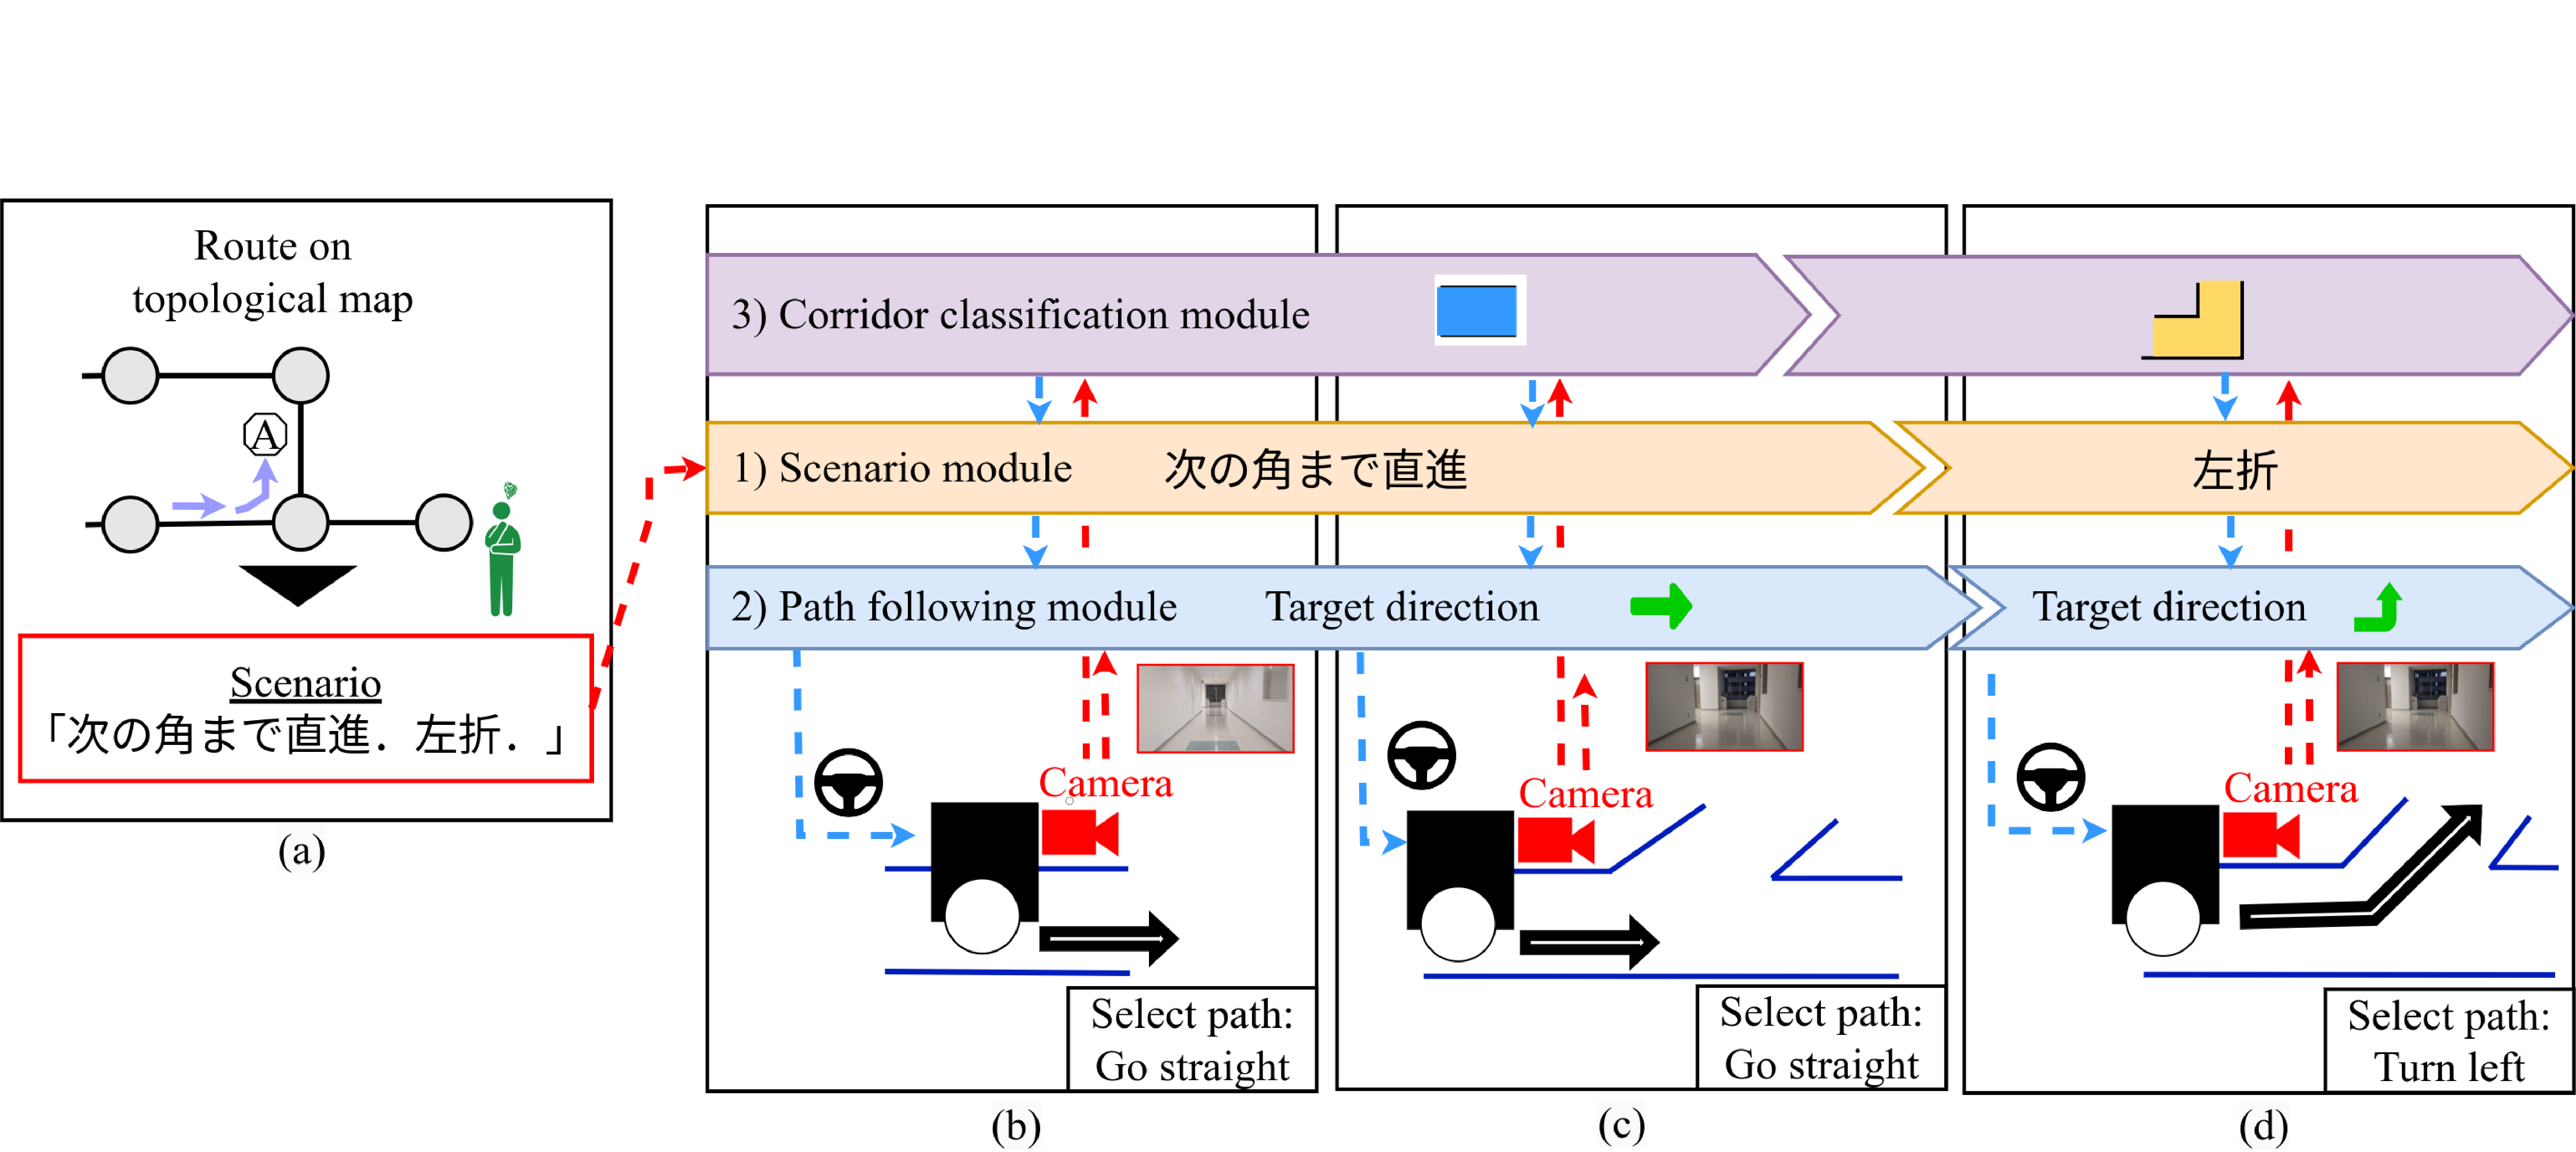
\includegraphics[width=130mm]{images/pdf/haruyama/system.pdf}
   \caption{Overview of proposed system (Quoted from \cite{haruyama2023})}
   \label{fig:sys}
\end{figure}

1)シナリオを分解し,「条件」と「行動」を抽出するモジュール(以後,シナリオモジュールと呼ぶ)

2)カメラ画像と目標方向を与えることで,経路を追従するモジュール(以後,経路追従モジュールと呼ぶ)

3)カメラ画像から通路の特徴を分類するモジュール(以後,通路分類モジュールと呼ぶ)

の3つのモジュールで構成される.ロボットは下記の a から d の一連の流れにより,指示された経路に沿って目的地まで自律移動する.
\begin{enumerate}
  \item [(a)] 
  トポロジカルマップ上の目的地に応じて,人間が「条件」と「行動」で構成されるシナリオを作成する.
  例えば,図のトポロジカルマップ上でAを目的地とするシナリオは「次の角まで直進.左折.」となる.
  \item [(b)] 
  作成したシナリオをシナリオモジュールへ入力する.
  シナリオモジュールは入力されたシナリオを分解し,「条件」と「行動」を抽出する.
  1つ目の条件と行動のセットは「次の角まで」と「直進」となる.
  この「直進」を目標方向として経路追従モジュールへ与える.
  経路追従モジュールは,カメラ画像と与えられた目標方向に基づいて,経路に沿って直進する.
  \item [(c)] 
  ロボットが角に近づくと,通路分類モジュールがカメラ画像に基づいて通路を「角」と分類し,それをシナリオモジュールに与える.
  シナリオモジュールはそれを基に「次の角まで」という条件を満たしたかを判定する.
  この場合は条件を満たしているため,2つ目の行動である「左折」へ遷移する.
  \item [(d)]「左折」に基づいて,経路追従モジュールは経路に沿って角を左折する.
\end{enumerate}

\subsubsection{シナリオモジュール}
シナリオモジュールは,トポロジカルマップを基に作成されたシナリオから「条件」や「行動」を解釈し,それを分岐路での目標方向に変換して出力する機能を持つ.
トポロジカルマップは,特徴的な通路のノード(青)とそれを繋ぐエッジ(緑)で構成され,ノードにはIDや通路の特徴,接続エッジと方向のデータが含まれている.
シナリオは目的地までの経路を「条件」と「行動」で表現し,例として「三叉路まで直進.右折.突き当たりまで直進.停止」となる.

シナリオの目標方向への変換では,句点ごとに分解し,「条件」と「行動」を抽出して以下の項目に分類する.
\begin{enumerate}
  \item [1)] 通路の特徴 (例:「三叉路」「角」)
  \item [2)] 順番 (例:「3 つ目の」「2 番目の」) 
  \item [3)] 方向 (例:「左手に」「右手に」)
  \item [4)] 行動 (例:「右折」「停止」)
\end{enumerate}

\figref{fig:scenario}に示す例で,「三叉路まで直進」は通路の特徴「三叉路」と行動「直進」に分解される.
この処理を経路全体に対して行い,得られた「行動」を分岐路での目標方向として変換し,経路追従モジュールに渡す.
また,条件の判定には通路分類モジュールを使用する.

\begin{figure}[htbp]
  \centering
   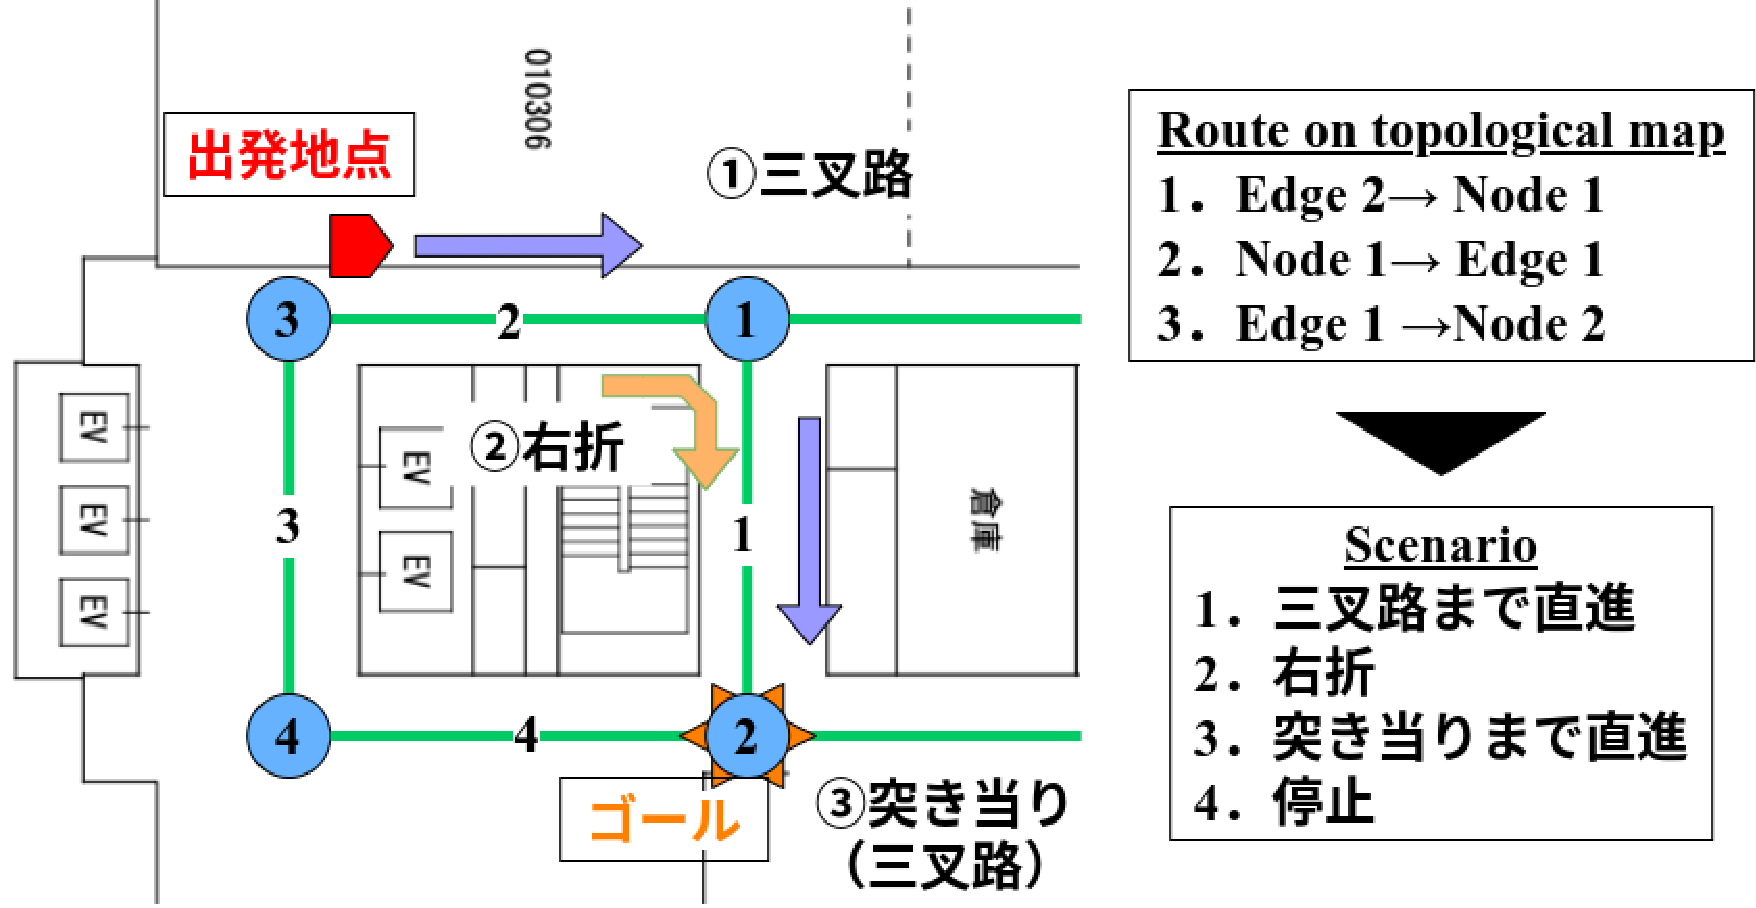
\includegraphics[width=130mm]{images/pdf/haruyama/scenario.pdf}
   \caption{ Example of topological map and created scenario Quoted from \cite{haruyama2023}}
   \label{fig:scenario}
\end{figure}

\clearpage
\subsubsection{経路追従モジュール}
このモジュールは,岡田らの手法から目標方向のデータを加えることで,分岐路で経路を選択し,移動する機能を追加したものである.
ここで目標方向とは,目標とする進行方向(「直進」や「右折」)を表す.
学習時は,カメラ画像とルールベース制御器が出力するヨー方向の角速度,目標方向を 0.2 秒周期でデータセットに加える.
データセットから抽出するバッチサイズや,カメラ画像の解像度は岡田ら手法と同様である.
データセットの収集には藤原ら\cite{fujiwara2023}が提案した,\figref{fig:oversample}に示す,データセットに加えるデータの不均衡を改善する手法,\figref{fig:behavior}に示す,学習時に積極的な蛇行する手法を採用する.

\begin{figure}[htbp]
  \centering
  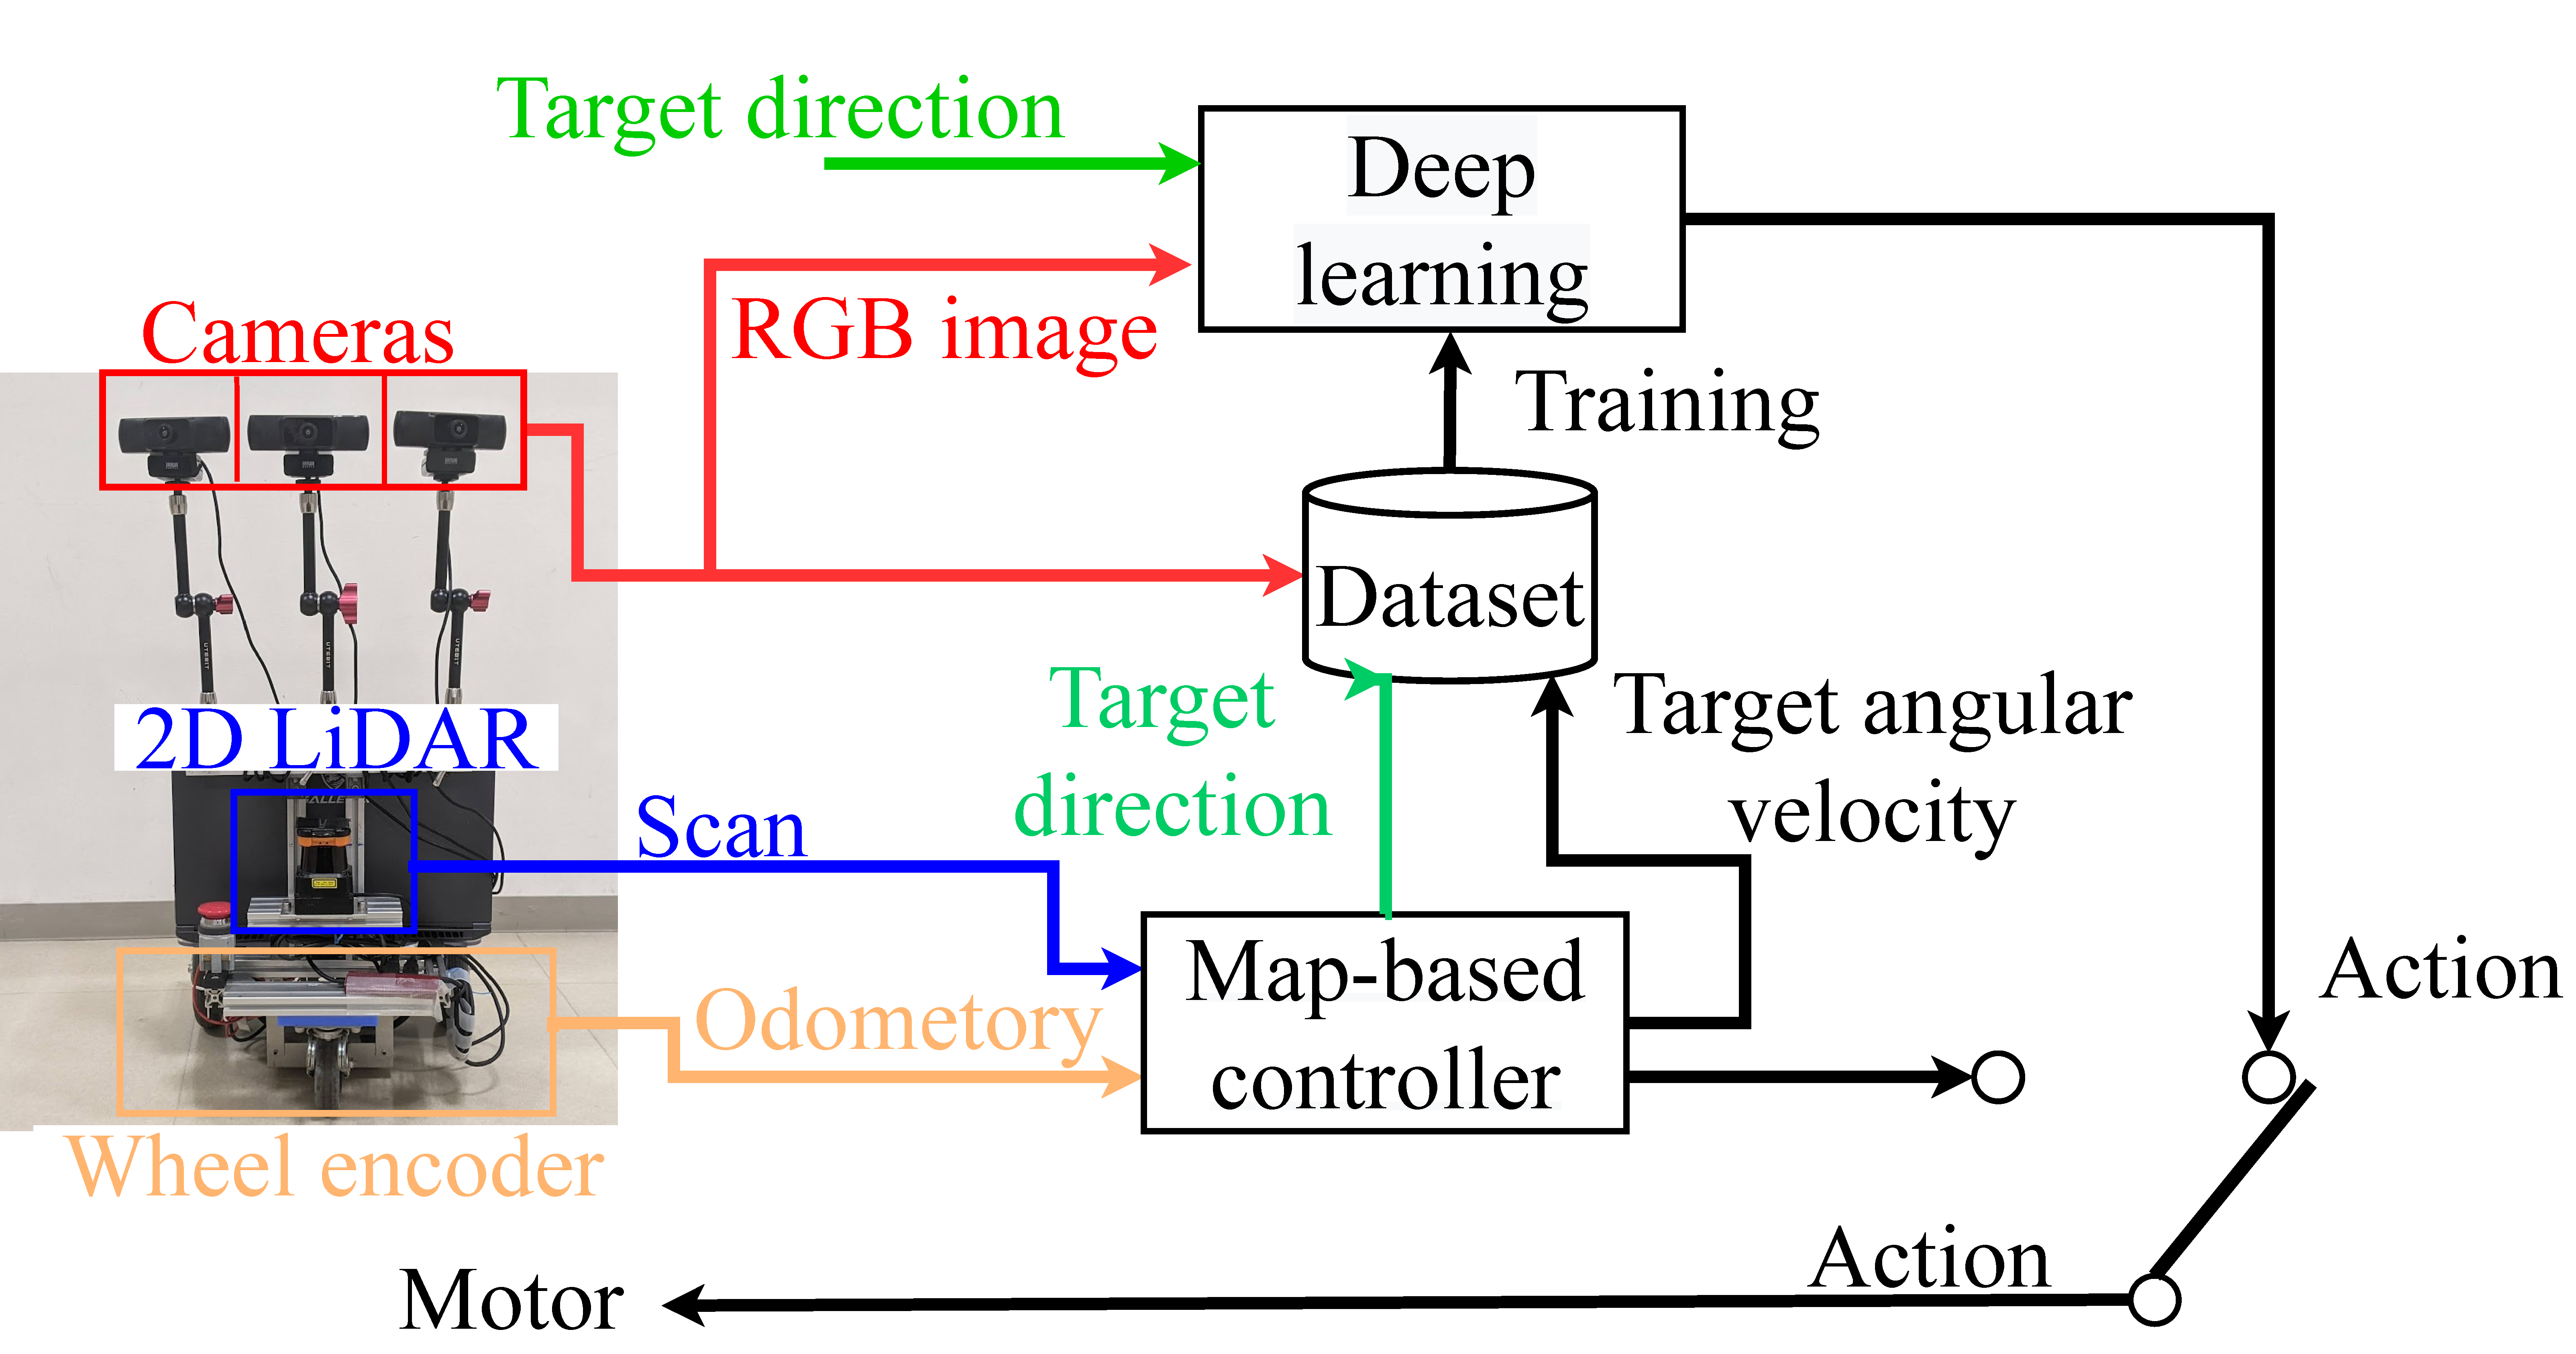
\includegraphics[width=100mm]{images/pdf/haruyama/pathfollow_sys.pdf}
  \caption{Path-following module system (Quoted from \cite{haruyama2023})}
  \label{fig:pathfollow}
\end{figure}

\begin{figure}[htbp]
  \centering
  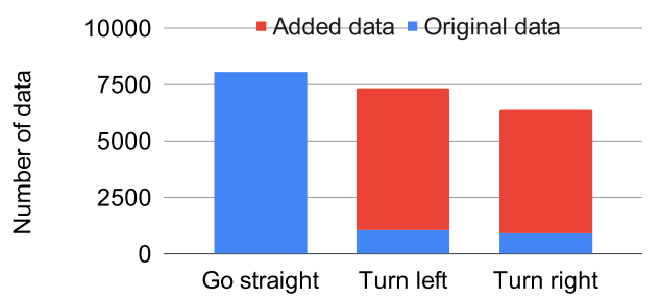
\includegraphics[width=100mm]{images/pdf/haruyama/oversample.pdf}
  \caption{Number of data in the target direction per 10000 steps in the previous 
  experiment(Quoted from \cite{fujiwara2023})}
  \label{fig:oversample}
\end{figure}

\begin{figure}[htbp]
  \centering
  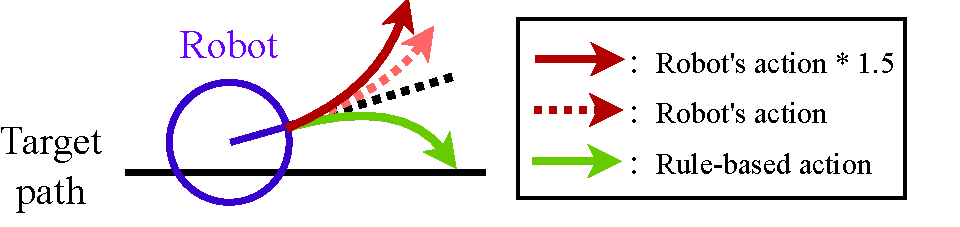
\includegraphics[width=100mm]{images/pdf/haruyama/behavior.pdf}
  \caption{Aggressive meandering(Quoted from \cite{fujiwara2023})}
  \label{fig:behavior}
\end{figure}

\subsubsection{通路分類モジュール}
このモジュールでは,ニューラルネットワークを用いることで,カメラ画像を入力として,通路の特徴を分類する.
データセットの収集をするために,ロボットをルールベース制御器に基づいて走行させる.
その際に,フレーム数 16 ,画像サイズ 64 × 48の連続したカメラ画像と通路の分類ラベルを1組として,0.125 秒周期でデータセットに加える.
通路の分類ラベルのアノテーションはルールベース制御器から出力されるラベルによって自動的に行う.
データセット内の不均衡を改善するために,クラス間のデータ数によって重み付けを行うコストアプローチを導入している.

\begin{figure}[htbp]
  \centering
   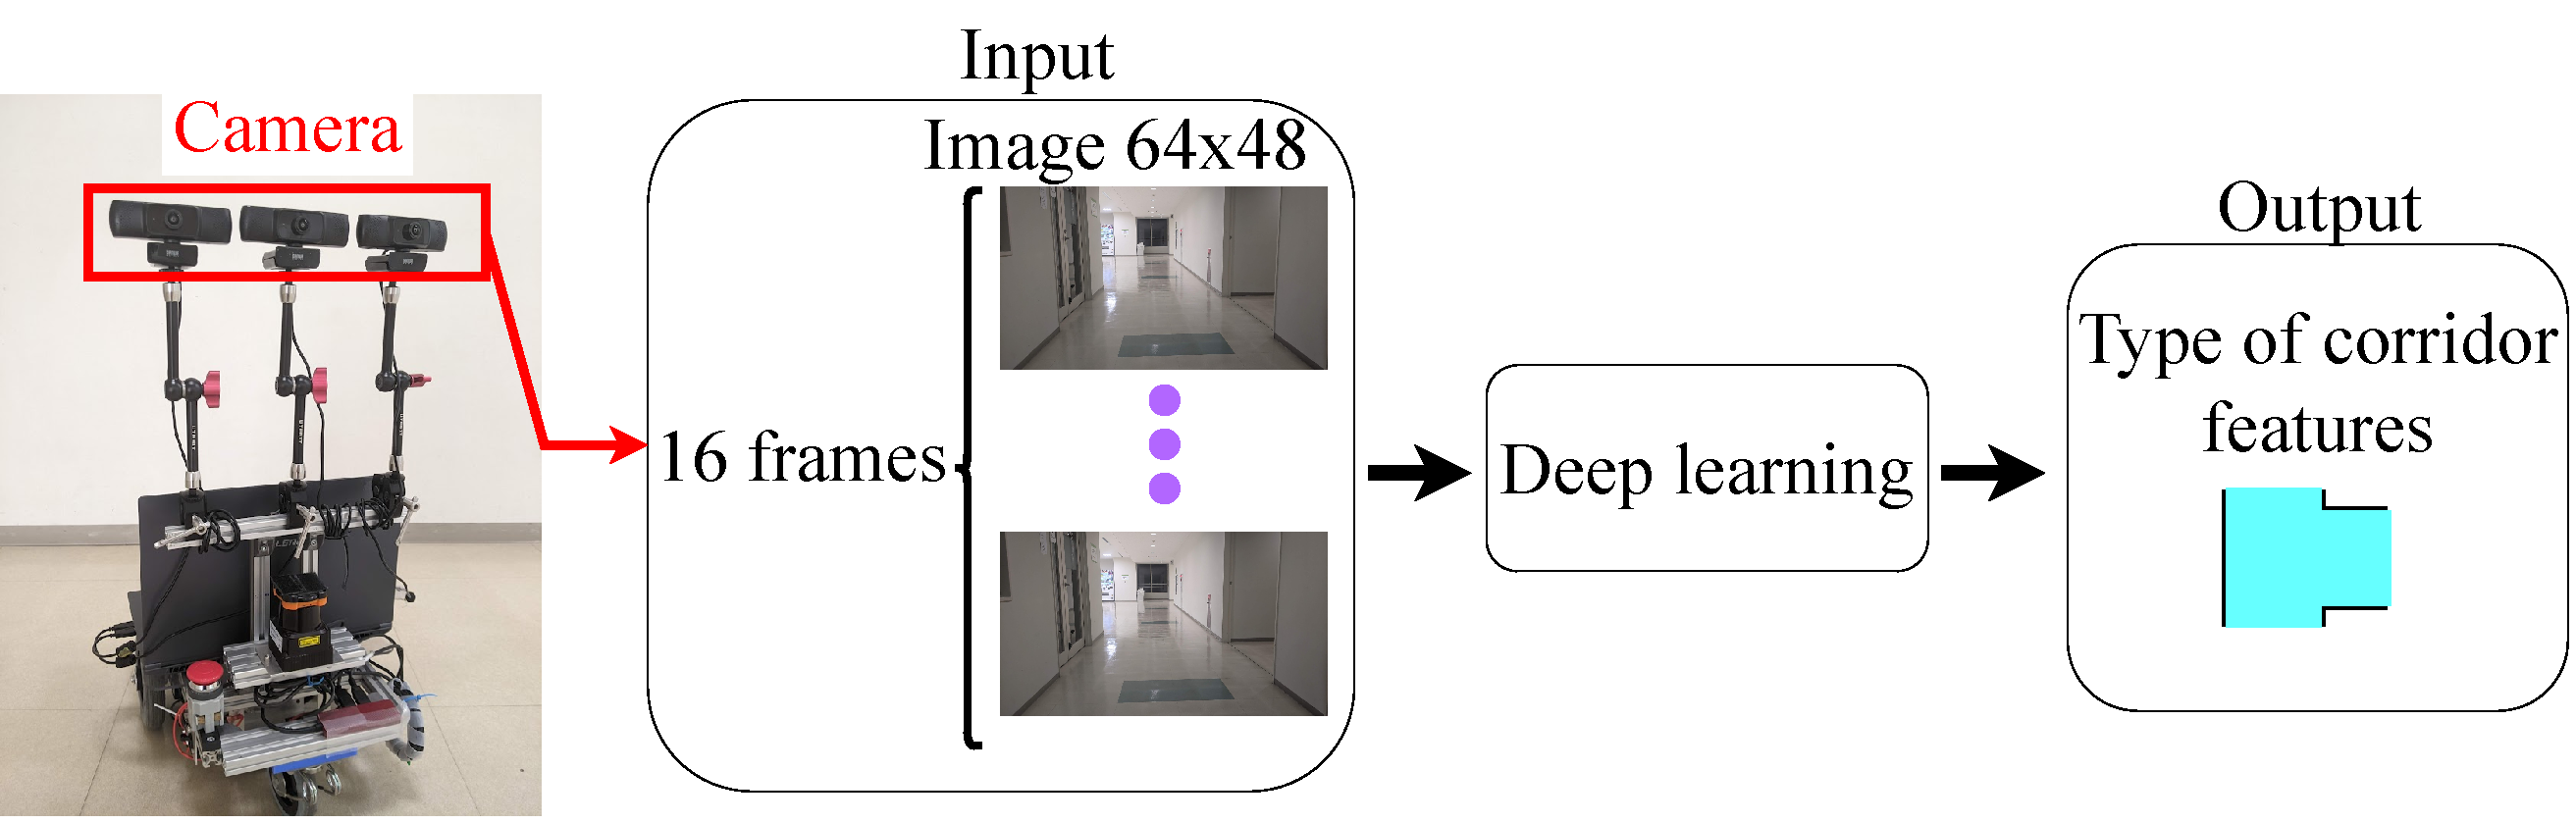
\includegraphics[width=130mm]{images/pdf/haruyama/intersection_sys.pdf}
   \caption{Path-following module system Quoted from \cite{haruyama2023}}
   \label{fig:intersection}
\end{figure}

\subsubsection{実ロボットを用いた実験}
実ロボットを用いた実験により,ロボットを目的地まで到達可能か検証されている.
実験では島田ら用いた 50 例のシナリオの中から,7例が用いられており,そのすべてでロボットが目的地へ到達できることが確認されている.